\chapter*{Introduction}\label{chapter:introduction}
\addcontentsline{toc}{chapter}{Introduction}

{
    The massive urbanization waves of the 20\textsuperscript{th} century has a bipolar effect on cities and city-planning mechanisms worldwide. On the one hand, urbanization created economic opportunities, reduction of poverty, agglomeration of knowledge and innovation, improved public health, and sustainable energy consumption, amongst many other benefits \cite{Glaeser2011, reckien2017climate, banerjee2011companion}. On the other hand, massive urban migration, entangled with climate change, technological disruptions, and inequality, challenge, and can even reverse the benefits of urban agglomeration \cite{parnell2016defining, reckien2017climate}. With projected two-thirds of world population living in cities by the mid-century, decision-makers and city-planning practitioners face these unprecedented challenges with outdated coping mechanisms \cite{united2018world, UnitedNationsHabitatIII2017}. Amidst these challenges, legacy planning processes are rendered insufficient \cite{Ben-Joseph2004, green2019smart, gaffney2018smarter}: Slow moving bureaucracy lag behind rapid population growth; monolithic regulations struggle with technological disruptions; scarcity of data and evidence-based processes stifle decision-making \cite{world2016inspiring, grauman1976orders, chen2014global}. These issues result with urban development patterns that fail to provide the basic needs of well-functioning cities \cite{Glaeser2011, banerjee2011companion}.
    \newline
    During the last two decades, several industries recognized these challenges, and sought to replace legacy urban processes with rapid, scalable, data-driven and evidence based solutions \cite{green2019smart, soderstrom2014smart}. Titled `Smart Cities', these efforts aimed to optimize urban environments using strategies, technologies, and methods inherited from the technology sector. Yet despite their promise, after two decades of real-world experiments, the majority of `Smart Cities' use-cases failed to offer real solutions to cities, rather than sporadic optimizations to legacy systems \cite{green2019smart, Hollands2008}. In most cases, these technological solutions often overlook the complexity of cities, and the ever-changing needs, behaviors, and dynamics of their inhabitants \cite{gaffney2018smarter}. Moreover, many Smart Cities solutions surfaced new concerns such as bias, inequality, privacy, and data-misuse \cite{green2019smart, Hollands2008}.
    \newline
    In this respect, both traditional urban processes, as well as techno-centric solutions, struggle to efficiently respond to the emerging challenges of 21\textsuperscript{st} century urbanization \cite{soderstrom2014smart,UnitedNationsHabitatIII2017, Hollands2008}. This thesis examines an alternative model for urban decision-making, that aims to take the best of both traditional processes and new solutions; It merges systematic, scalable, evidence-based and data-driven planning, with a comprehensive, long-term, and community-driven discourse. This \textit{New Urban Process}, is manifested in the design, development and deployment of \textbf{CityScope}: an urban modeling, simulation, and decision-making platform, that marries urban technology with social discourse. This thesis clusters a series of lab experiments and real-world deployments of the CityScope platform into four major themes: Insight, Transformation, Prediction, and Consensus (see Chapters \eqref{ch:insight}, \eqref{ch:transformation}, \eqref{ch:prediction}, and \eqref{ch:consensus}).
    \newline
    The rest of this chapter discusses the need for a new urban process, through an overview of the state of global urbanization trends, their challenges, and leading mitigation efforts. It then discusses the evolution of collaborative, data-driven approaches to city-planning, and it concludes with an overview of CityScope's role in a new urban process.
}


\section{The State of Cities}\label{sec:stateofcities}
{
    Since 2005, over 50\% of the world population is estimated to live in urban areas; Projections are that around 70\% will occupy cities by 2050 \cite{united2018world}. In comparison, urban growth rates of the past three decades (\%39-\%50) are nearly equal to the entire trend of urbanization between 1650 - 1900, (\%5.9-\%18) \cite{grauman1976orders, chen2014global}. This unprecedented move to densely-populated areas met with planning mechanisms that are incapable of adequately address rapid growth \cite{Glaeser2011, united2018world}. When urbanization trends are not adequately mitigated, many of the advantages of urbanization might dissolve or even reverse \cite{chen2014global}. This section discusses the evolution, and current state of city-planning amidst urbanization challenges.


    \subsection{Traditional Planning Processes}
    {
        A consolidated, structured, and holistic process of city-planning emerged in the early 1920's \cite{banerjee2011companion}. The waves of urbanization during the the 19\textsuperscript{th} century, and the impacts of the industrial revolution on urban growth, wealth, and well-being, created the need for a balanced distribution of land resources, and the mitigation of development pressure \cite{Glaeser2011}. As Birch argues, the idea of building a modern, rationally ordered city, captured the imaginations of both designers and regulators, who saw an opportunity to establish a due urban process. Regulated planning processes have strongholds in law, government, and industries, thus making them systematic and fairly stable, but also difficult to amend and hard to improve \cite{banerjee2011companion}.

        \subsubsection{Planning for Extreme Growth}
        {
            Since the turn of the century, unprecedented urbanization, technological disruptions, and economic turmoil, increasingly grew the pressure on traditional planning mechanisms. In places where slowly moving planning trailed rapidly expanding cities, alternative, in-formal, and ad-hoc models of urbanization started to emerge \cite{UnitedNationsHabitatIII2017}. Housing shortages, lack of amenities, and inadequate infrastructure, forced stakeholders to favor hyper-localized solutions in-lieu of more holistic strategies \cite{banerjee2011companion}. This sort of patchwork urbanism surrounds the historical cores of many well established cities. They might adapt relatively high-density and seemingly `urban' characteristics, but will often lack proper land-use mixity, amenities, and distribution of resources, commonly known as `commuter towns' \cite{united2018world, UnitedNationsHabitatIII2017}. In the developing world, where informal settlements and rapid-urbanization strived for pre-made solutions, these planning models were quickly adapted, with minimal adherence to context and local factors \cite{reckien2017climate}.
        }

        \subsubsection{Planning Stagnation}
        {
            The slow pace of traditional planning processes has also negative impacts on the resiliency of urban systems. As Scheer argues, the urban landscape, as any evolving system, requires flexibility and elasticity to accommodate change over time \cite{banerjee2011companion}. Static regulatory systems would not be resilient to outside forces, and would often struggle with changing economics and technological disruptions. Despite flagging these concerns several decades ago, static tools, such as rigid master-planning, are still central in traditional urban processes \cite{banerjee2011companion, UnitedNationsHabitatIII2017}. As Talen argues, over the course of the last century, urban-planning moved away from the creation of constructive design guides, to wordy policy documents, thus producing misunderstandings, foot-dragging, and undesired outcomes \cite{banerjee2011companion}.
        }
        \subsubsection{Evidence-Based Planning}
        {
            Despite the growing incorporation of scientific processes in daily life, planning is still not fully accompanied by evidence-based and data-driven decision-making. Most contemporary urban research lacks necessary scientific background, and is ill-prepared to interact with changes in global policy \cite{McPhearson2016, habitat2016new, Inostroza2015}. Decision-makers suffer from scarcity of data and evidences, and are not able to effectively assess changes as they occur \cite{bulmer_how_2001}. Even when science is part of the process, it is usually incorporated in an inaccessible manner. As McPhearson mentions, to be useful to policymakers, urban research must be organized, representative and seen as legitimate \cite{McPhearson2016}.
        }
    }

    \subsection{Mitigating Mass-Urbanization}
    {
        As the challenges associated with mass-urbanization became more apparent, global stakeholders began devising policies in an effort to mitigate the risk. These efforts focus on global challenges, while setting concrete road-maps and goals for local authorities. This Section presents some of the prevailing efforts to address urbanization challenges, with an emphasis on the creation of new urban processes.

        \subsubsection{The New Urban Agenda}
        {
            In 2016, UN-HABITAT - the United Nations urban development arm, organized a global development summit called Habitat III. The summit was concluded with the inauguration of a report titled the `New Urban Agenda" (NUA) \cite{habitat2016new}, a list of establishing principles for global development in the next two decades. In over 200 design and development items, the NUA urges member states to address the challenges and impacts of mass-urbanization: \textit{``in this unprecedented era of increasing urbanization...If well-planned...urbanization can be a powerful tool...for both developing and developed countries"} \cite{habitat2016new}. Specifically, the NUA calls for new models of city-planning that are fexible and agile enough to confront the rapid evolution of cities.
            \newline
            In terms of technology, the NUA promotes the usage of new tools, methods, and systems to create an evidence-based planning model: \textit{``...We will promote...the use of digital platforms and tools, including geospatial information systems...to improve long-term integrated urban and territorial planning and design, land administration and management, and access to urban and metropolitan services.''}
            The NUA also calls for the integration of planning mechanisms that can better predict the impacts of development: \textit{``We will...(be) providing predictability and coherence in urban development plans to enable social inclusion, sustained, inclusive and sustainable economic growth and environmental protection.''} Lastly,
            it urges decision makers to support collaborative development that empowers communities, their needs, and their goals by promoting the usage of participatory processes: \textit{``...We will promote participatory...approaches at all stages of the urban and territorial policy and planning processes...using information and communications technologies and accessible data solutions.''}
        }

        \subsubsection{UN-SDG17}\label{subsec:un-sdg}
        {
            The UN ``2030 Agenda for Sustainable Development" (SDG-17) \cite{assembly2015transforming} are 17 high-level goals designed to be a \textit{``blueprint to achieve a better and more sustainable future"} \cite{assembly2015transforming}\footnote{The SDGs were devised by the United Nations General Assembly in 2015 and are intended to be achieved by 2030. A lists of targets and indicators for each of the SDGs was published in a UN resolution in 2017}. Each goal typically has 8 to 12 targets, and each target has between 1 and 4 indicators used to measure progress. The dual model of goals and indicators has several advantages: The usage of measurable indicators bounds actionable progress to implicit goals. It is also inviting novel methods of data collection, analysis, visualization and communication, that boost traditional processes with modern methods \cite{Klopp2017}.
            \newline
            SDG-17 sets goals not only for future developments, but also for future urban-planning processes. For example, SDG $11.a$ seeks to \textit{``Make cities and human settlements inclusive, safe, resilient and sustainable''} by strengthening national and regional development planning. SDG $11.a$ is evaluated by indicator $11.a.1$, measuring the number of countries that have national urban policies or regional development plans that (i) respond to population dynamics; (ii) ensure balanced territorial development; and (iii) increase local fiscal space. In parallel, SDG $11.3$ promotes the enhancement of \textit{``inclusive and sustainable urbanization and capacity for participatory, integrated and sustainable human settlement planning''}. This SDG is indicated in part by the \textit{``Proportion of cities with a direct participation structure of civil society in urban-planning and management that operate regularly and democratically''} \cite{assembly2015transforming}. As with the NUA, the SDGs seeks to revisit the urban process itself, by addressing new planning, design, and collaboration processes.
        }

        \subsubsection{IPCC Report on Climate Change}
        {
            The growing concerns around the impacts of human activities and climate change motivated the creation of several international research, policy, and mitigation projects. The WMO's and UNEP's IPCC\footnote{The Intergovernmental Panel on Climate Change is the United Nations research and knowledge-sharing body on climate change, internationally accepted by most member states \cite{shukla2019ipcc}. Twice a decade, the IPCC releases an Assessment Report which motivates member states to acknowledge and address the impacts of climate change. AR6 Synthesis Report (SYR), which comines the IPCC three Working Groups (WG) will be the last of the AR6 products, due for release in 2022.} reports dedicated significant portions to the relationship between urban development, land-use, and the design of cities and urban systems, to their impact on GHG (Greenhouse Gasses), climate change, and environmental issues. The IPCC clearly concludes that in order to avoid global warming of additional 1.5°C \textit{``rapid and far-reaching transitions in energy, land, urban and infrastructure..., and industrial systems.''}\cite{allen2019technical} are required. The Fifth and Sixth Assessment Report (AR5, AR6) include chapters on \textit{``Human Settlements, Infrastructure, and Spatial Planning''} which look into the impacts of current models of urban development on the world's carbon cycle. The reports finds that \textit{``Urban areas represent 67-72\% of global emissions''} and that \textit{``With 80\% of the global population expected to be urban by 2050, cities will shape development paths for the foreseeable future...How new cities and towns are designed, constructed, managed, and powered will lock-in behaviour, lifestyles, and future urban GHG emissions.''}\cite{IPCC_AR6_22}
            \newline
            \textbf{Climate and the Planning of Informality:} Specifically, the IPCC report highlights the emerging gaps between traditional, slow-paced and top-down practices of city-planning, and the rapid urbanization in informal settlements: \textit{``the most rapid growth in urban vulnerability ...(is) especially in unplanned and informal settlements in low- and middle-income nations...Between 2015 and 2020, urban populations globally grew by more than 397 million people, with more than 90 percent of this growth taking place in Less Developed Regions.''}\cite{IPCC_AR6_22} The report urges policymakers to rethink planning processes so that they could mitigate both rapid urbanization and growing environmental concerns: \textit{``The challenge for many policymakers is to construct development paths that make cities clean, prosperous and liveable while mitigating climate change...Urban planning reforms are therefore central to building a fairer urban adaptation response.''}\cite{IPCC_AR6_22} Nevertheless, the report also acknowledges that the planning of settlements in the next few decades will meet rapid and informal urbanization, thus requiring agile, flexible, and community driven strategies. These will have to emerge from a well coordinated effort between policies, stakeholders, governments, and communities: \textit{``The feasibility of spatial planning instruments for climate change mitigation is highly dependent on a city's financial and governance capability...a high level of coordination across institutions can increase the likelihood of achieving emissions reductions and avoiding unintended outcomes.''} \cite{shukla2019ipcc}
            \newline
            \textbf{Collaborative Climate Action:} The IPCC includes actionable recommendations for creating a comprehensive, long-term, and community driven process: \textit{``These goals will reflect the specific challenges facing individual cities and local governments...as key factors: (1)...mitigation with other high-priority urban agendas; (2) a multilevel governance context that empowers cities to promote urban transformations; (3) spatial planning competencies and political will to support integrated land-use and transportation planning.''} Similar to the SDGs (see Section \eqref{subsec:un-sdg}), the IPCC approach to spatial planning and decision-making is based on the need for flexible, adaptive, and collaborative planning processes: \textit{``A characteristic of effective spatial planning is interlinked and coordinated efforts that are synergistic...Relying on a single instrument or one-size-fits-all approach can be ineffective or worse...Bundling spatial strategies in ways that produce positive synergies often requires successful institutional coordination and political leadership...''}
            \newline
            \textbf{Climate as Part of an Holistic Agenda:} The IPCC values not only the outcomes of positive urban development models, but also processes that can be used to address the challenges of city-planning in times of climate change. In parallel to other urban mitigation efforts\cite{habitat2016new, Klopp2017}, the IPCC sees climate action as only one aspect in a positive urban development effort: \textit{``Adaptation actions will be more effective if they are implemented in partnership with local communities, national governments, research institutions, and the private and third sector. Climate action should not be considered as an additional or side action to other activities. Rather, climate action should be mainstreamed into existing processes...''}\cite{IPCC_AR6_22}
        }

        \subsubsection{ESG Metrics for Real-Estate}
        {
            Environmental, Social and Governance (ESG) metrics were created during the last two decade in order to evaluate companies operations, and offer investors empiric means to screen potential investments \cite{friede2015esg}\footnote{The Environmental criteria consider how a company might perform in the context of natural resources, the environment, and climate change. The Social criteria examine how it manages relationships with employees, suppliers, customers, and the communities in which it operates. Governance deals with leadership, executive pay, audits, internal controls, and shareholder rights.}. In the context of the built environment, ESG are used to evaluate the rehabilitation of public spaces, affordable and social housing, or through environmental investments, such as green buildings and sustainable development \cite{deloitte_2021}\footnote{Some of the more common ESG reporting frameworks for real-estate are (i) GRESB (Global Real-estate Sustainability Benchmark), a measures of ESG performance metrics; (ii) the aforementioned SDGs, designed to be a measurable tool for global development efforts; additional UN standard is (iii) GRI, a modular framework focusing on activity areas within the lifecycle of a building; (iv) CDP (Carbon Disclosure Project), a climate impacts disclosure system used by investors, companies, and governments; (v) PRI (Principles of Responsible Investment) which encourages companies to become annual voluntary signatories, submitting responsible investment activities for review and assessment reporting; and (vi) SASB (Sustainability Accounting Standards Board), a set of sustainability standards for real-estate owners, developers, and investment trusts to asses energy, water, management of tenant sustainability impacts, and climate change adaptation \cite{swl2021}.}.
            In recent years - and especially due to the social and economic turmoil following the COVID-19 pandemic - new emphasis was given to the Social aspect of ESGs, in order to asses the long-term societal benefits of urban development. Given its more implicit nature, the social aspect of ESG is less often assessed, and the need for new metrics and better evaluation methods has increased \cite{swl2021}. With more emphasis on ESG adherence in real-estate, new tools, methods, and frameworks to assess ESG performance in planning processes will also increase.
        }
        \newline
        A common-ground between the different mitigation efforts mentioned above, is the search for alternative processes of planning and evaluation. Amidst these efforts, looming the need for a more integrated approach to urban development, that can accommodate many of these ideas into a comprehensive process. The next section discuss the state of the art efforts to create new planning systems, tools, and processes.
    }
}

%%%%%%%%%%%%%%%%%%%%%%%%%%%%%%%%%%%%%%%%%%%%%%%%%%%%%%%%%%%%%%%%%%%%%%%%%%%%

\section{Towards a New Urban Process}

 {
  As described in section \eqref{sec:stateofcities}, contemporary urban processes are still heavily fragmented and inconsistent \cite{branch1978critical, banerjee2011companion, Ben-Joseph2004}. Even when cities attempt to modernized their processes, scarcity of data and inaccessibility to modeling, simulation, and analysis methods hinder evidence-based planning efforts \cite{UnitedNationsHabitatIII2017, banerjee2011companion}. To address some of these challenges, alternative urban decision-making began to emerge in recent decades \cite{ben-joseph2001, Ishii2002, banerjee2011companion, Snyder2003, mueller2018citizen}. The following sections review six decades of efforts to create alternative planning systems, urban human-computer platforms, and collaboration processes.
 }

\subsection{Collaborative Urban Processes}

{
    The legal framework empowering public participation in city-planning, dates back to the 1950's \cite{banerjee2011companion}. Many early attempts to involve `non-experts' were later criticized for their lack of transparency, politicization, and privatization \cite{Innes2016}. As Arenstien argues, the regulatory enforcement of institutionalized participation, paradoxically reduced the ``citizen power'' to mere tokenism \cite{arnstein1969ladder}. Today, most large-scale planning initiatives would not be held successful without some consent of the general public. Consensus making has become critical in complex planning processes, where opinionated and well-informed public is invested in the process: \textit{``...we have seen the continued growth of public engagement in government decision-making; partly in response to demands for `more democracy' and partly as a pragmatic step aimed at building public support for the actions of elected and appointed officials.''} \cite{susskind1984mediated} Nevertheless, the efforts to create a meaningful public discourse are still limited: \textit{``...too many government agencies fail to pursue these requirements in an effective manner. They go through the motions, hunkering down to defend decisions rather than engaging stakeholders in a timely and meaningful way.''} \cite{susskind1984mediated}
    \newline
    In recent years, the need for new participation models grew amongst both practitioners and knowledgeable citizens. This model was expressed by the NUA: \textit{``We will foster the creation (...) of tools available to transfer and share knowledge.''} \cite{habitat2016new}
    If the effort to `transfer and share knowledge' is successful, it can promote `citizen experts', armed with access to information, planning and design knowledge, who act as proactive public participants \cite{banerjee2011companion}. The usage of new participatory processes that are inherently open for interpretation and critical review, can also create what Innes describes as `Collaborative Participation'. Collaborative Participation emerges when joint fact finding is conducted by parties who can question not only the results of a processes but also the data, models and the process itself \cite{Innes2016}.
}

\subsection{The Emergence of UHCI}\label{subsec:emergence_uhci}

{
    The NUA effort to create an \textit{"open, user-friendly and participatory data platforms"} can be found in the design, development, and deployment of many socio-technical planning systems in recent decades \cite{batty2013new, ben-joseph2001}. Since the 1960's, \textbf{Urban Human-Computer Interaction} (UHCI) research embraced the idea of open, collaborative, and iterative design environments, engaging professionals and non-professionals alike in city-planning discourse \cite{Ben-Joseph2004, Ishii2008}.


    \begin{figure}[h]
        \begin{center}
            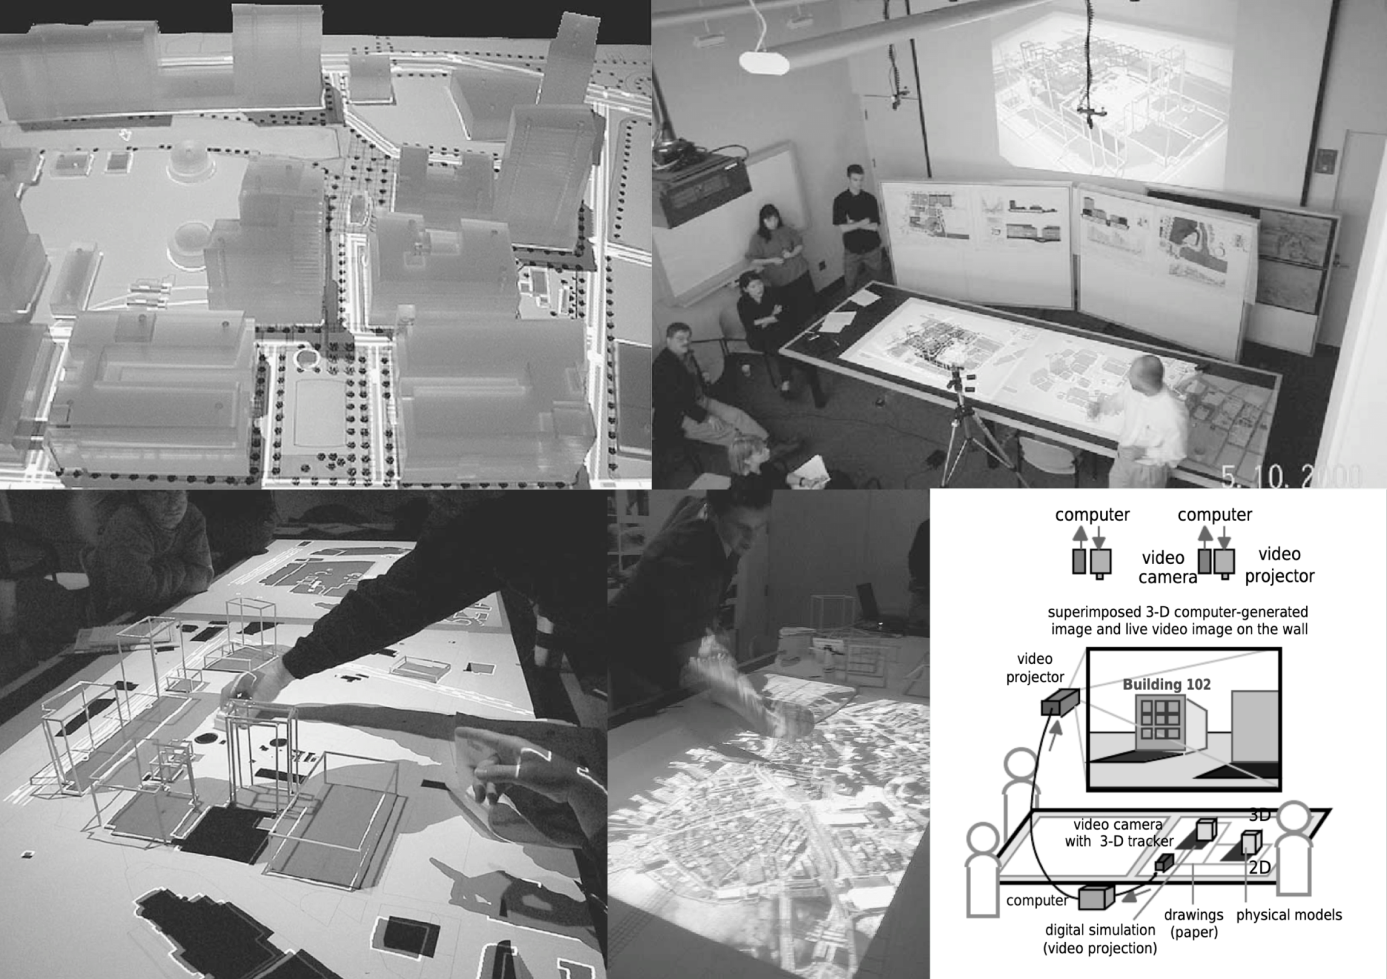
\includegraphics[width=1\textwidth]{chapters/introduction/figures/ebj.png}
        \end{center}
        \caption{Ben-Joseph, "luminous planning table" (2001) \cite{ben-joseph2001}}
        \label{fig:luminous}
    \end{figure}


    Although different in their design or usage, many of these UHCI platforms, as well as most CityScope instances, are modeled after Snyder's `13-points for urban-design tools': (1) interactive and usable at multiple levels of expertise; (2) accessible and affordable; (3) adaptable and maintainable; (4) designed with open architecture; (5) utilizing high quality data; (6) operating at local and regional scale; (7) providing comprehensive coverage and integration of issues; (8) supporting impact analysis including short, medium and long-term effects; (9) engaging citizens and supporting face-to-face interactions; (10) visual imagery; (11) values, causes, and effects; (12) promoting identification of design options; (13) and regular monitoring and reporting \cite{Snyder2003}.
    \newline
    The following sections cluster these UHCI principals into three main categories:
    (i) their design supports multi-stakeholders and collaborative decision-making; (ii) they promote playful, iterative, and real-time design and feedback-loops; and (iii) they are easy to use, interactive, vividly visual, and tangible in nature \cite{Ullmer2010, ben-joseph2001, Snyder2003, mueller2018citizen}.

    \subsubsection{(i) Multi-Stakeholders}
    {
        A key aspect of UHCI is the engagement of many stakeholders at once \cite{Ben-Joseph2004}. Unlike traditional design systems, these platforms are built around shared spaces (physical or virtual) that can facilitate many participants, while reducing the mental and bureaucratic overhead of negotiating in different channels \cite{ben-joseph2001}. Several notable UHCI platforms were developed for collaborative urban-design: the Environmental Simulation Laboratory (ESL) in Berkeley \cite{bosselmann1984berkeley}, URP \cite{underkoffler1997view}, and the Augmented Urban-planning Workbench \cite{Ben-Joseph2004} (see Figures \eqref{fig:berkely_env_lab}, \eqref{fig:luminous}) were amongst the first to suggest alternative collaboration in the urban process\footnote{for a full list of prior art in UHCI, see Section \eqref{sec:uhci_catalog}}. With the growth of the internet, collaboration and participation were extended beyond the limits of physical spaces. Using virtual `sandboxes', planning discussions began to take place remotely, thus extending the number of potential participants in an order of magnitude \cite{Ben-Joseph2013, banerjee2011companion, green2019smart}. Advancements in Virtual, Augmented, and Mixed Reality, enhance the experience of remote participants to understand, discuss, and reach consensus using immersive environments \cite{bulmer_how_2001, noyman2018CityScopeARUD}.

        \begin{figure}[h]
            \begin{center}
                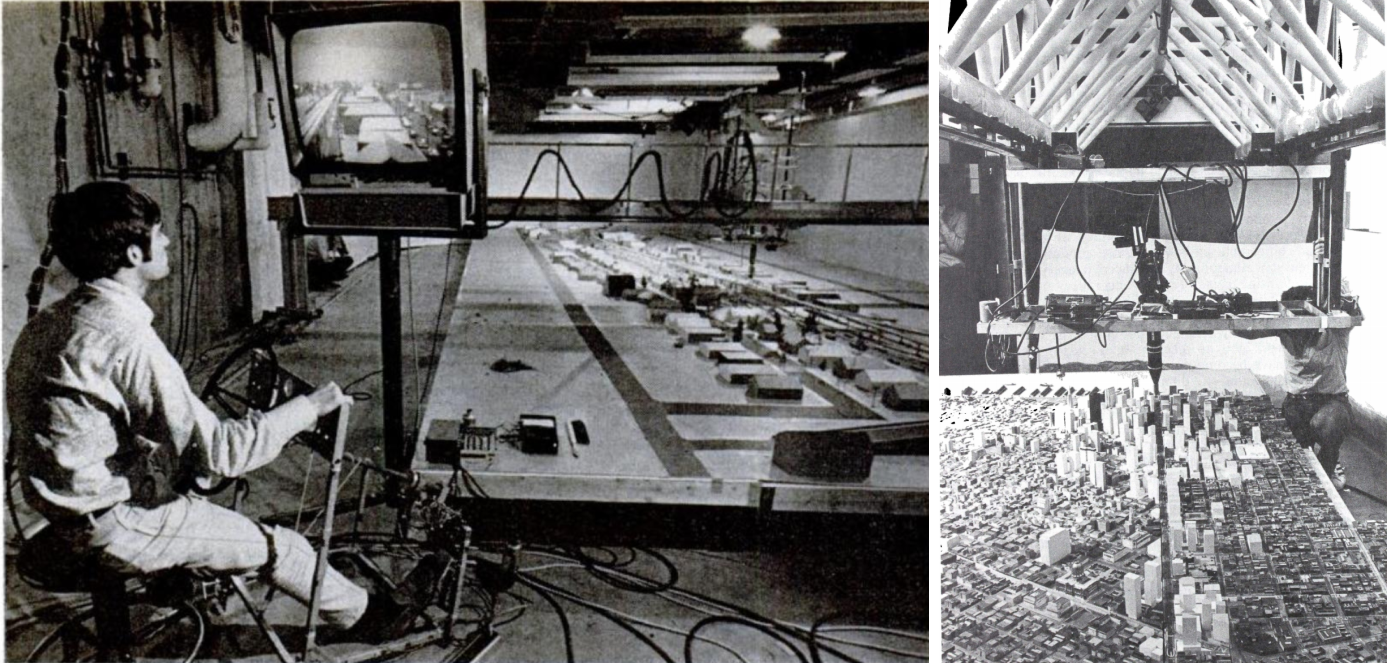
\includegraphics[width=1\textwidth]{chapters/introduction/figures/berkely_env_lab.png}
            \end{center}
            \caption{Bosselmann, ``The Berkeley Environmental Simulation Laboratory'' (1984) \cite{bosselmann1984berkeley}}
            \label{fig:berkely_env_lab}
        \end{figure}

    }

    \subsubsection{(ii) Iterative and Real-time}
    {
        To allow for an effective decision-making process, UHCI must adapt an iterative design process and real-time feedback. The latter is essential to the success of UHCI, as it allows for the rapid and efficient development of new solutions. Unlike traditional design processes, which often involve costly prototypes, models, drafts, or sketches, UHCI promotes a dynamic graph of potential design iterations, with minimal overhead and virtually no cost: \textit{``If the creative process is to be assisted by the computer, the machine has to act reciprocally and simultaneously to produce a smooth dialogue. For an urban-designer this conversation must be graphical. His entire training, practice and design process are graphical...''} \cite{Infoscapes} Prior art of real-time UHCI include the I/O Bulb, The Clay Table, and Sensetable \cite{Ishii2004, Ishii2002, Ishii2008}, which converged the digital and the physical in a seamless design-feedback loop. This kind of a synchronous design process does not only expedites the designer's work, but can also help expose edge-cases and design failures. Modern spatial analytics and urban-modeling techniques can serve UHCI platforms with real-time data and advanced insights \cite{Kitchin2014, salganik_bit_2017}. Data-driven modeling techniques, as well as Machine-Learning and Deep-Learning, can expedite the investigation of complex planning scenarios and their effects on human dynamics, traffic, energy-use, or economic performance \cite{Foth2011, doorley2019s, noyman2020deepscope}.
    }

    \subsubsection{(iii) Interactive, Visual, and Tangible}

    {
        Processes of urban-planning, design, and architecture are inherently tangible, as they deal with the tactility of the built environment. Models of building details and complex structural intersections were found in early construction sites, suggesting their usage as communication aids \cite{hewitt1985representational, Noyman2015power}. In the mid-20\textsuperscript{th} century, computational design systems began to reform the idea of `modeling': \textit{``in the early 1980's, CAD software started to gain widespread acceptance...It particularly gained momentum in 1988 with its first exploratory release of a three-dimensional modeling system. By the early 1990's, the technology for generating entire landscapes by computer was readily available to design and planning professionals.''} \cite{underkoffler1997view} Nevertheless, these new tools were not always suited for real-time and interactive usage: \textit{``...such simulations required time-consuming calculations to generate realistic lighting, reflections, and rendering details...While urban simulation programs have made steady progress in the past decade, they are still confined to two-dimensional flat interfaces. As such, they leave much to be desired.''} \cite{underkoffler1997view}
    }
    \newline
    The efforts to create alternative planning processes through the usage of novel interfaces and interactions, branched into many different UHCI solutions. The next section explores the emergence of some of these platforms and the way they supported a new urban-planning process.
}
%%%%%%%%%%%%%%%%%%%%%%%%%%%%%%%%%%%%%%%%%%%%%%%%%%%%%%%%%%%%%%%%%%%%%%%%%%%%


\section{Urban Human-Computer Interaction: A Catalog}\label{sec:uhci_catalog}

{
    This section reviews several key milestones of tangible, collaborative, and real-time design platforms. This list is focuses on methods that incorporated sharing and collaboration by design, more so than mere technological or computational advancements.

    \subsection{Tangible Design Systems}
    {
        The following projects focus on finding common grounds with stakeholders and communities, by distilling complex urban problems using simple physical objects. \textit{The Center for Urban Pedagogy (CUP)} \cite{menking2009center} is a nonprofit organization that uses design and art to improve civic engagement in urban-planning. CUP projects discuss urban policy and planning issues using physical game-like tools. The main goal of CUP is to establish pedagogic channels that offer uniformed communities a chance to understand their physical and legal surroundings. Similarly, \textit{Place it!} \cite{HumanCit17:online} is a design and participation practice that uses model-building workshops to help engage the public in the planning process. Through its sessions, participants are able to learn about the role of planning and design in shaping cities, and to translate ideas into forms and models. Lastly, \textit{Game Urbanism} \cite{venhuizen2010game} examines the structure of game playing and applies it to spatial planning and collective decision-making processes. The relation between playfulness and seriousness is a key, as the game simplifies complex situations by revealing the wishes and interests of involved parties.
    }
    \subsection{Software And Web-Based Collaboration}
    {

        \begin{figure}[h]
            \begin{center}
                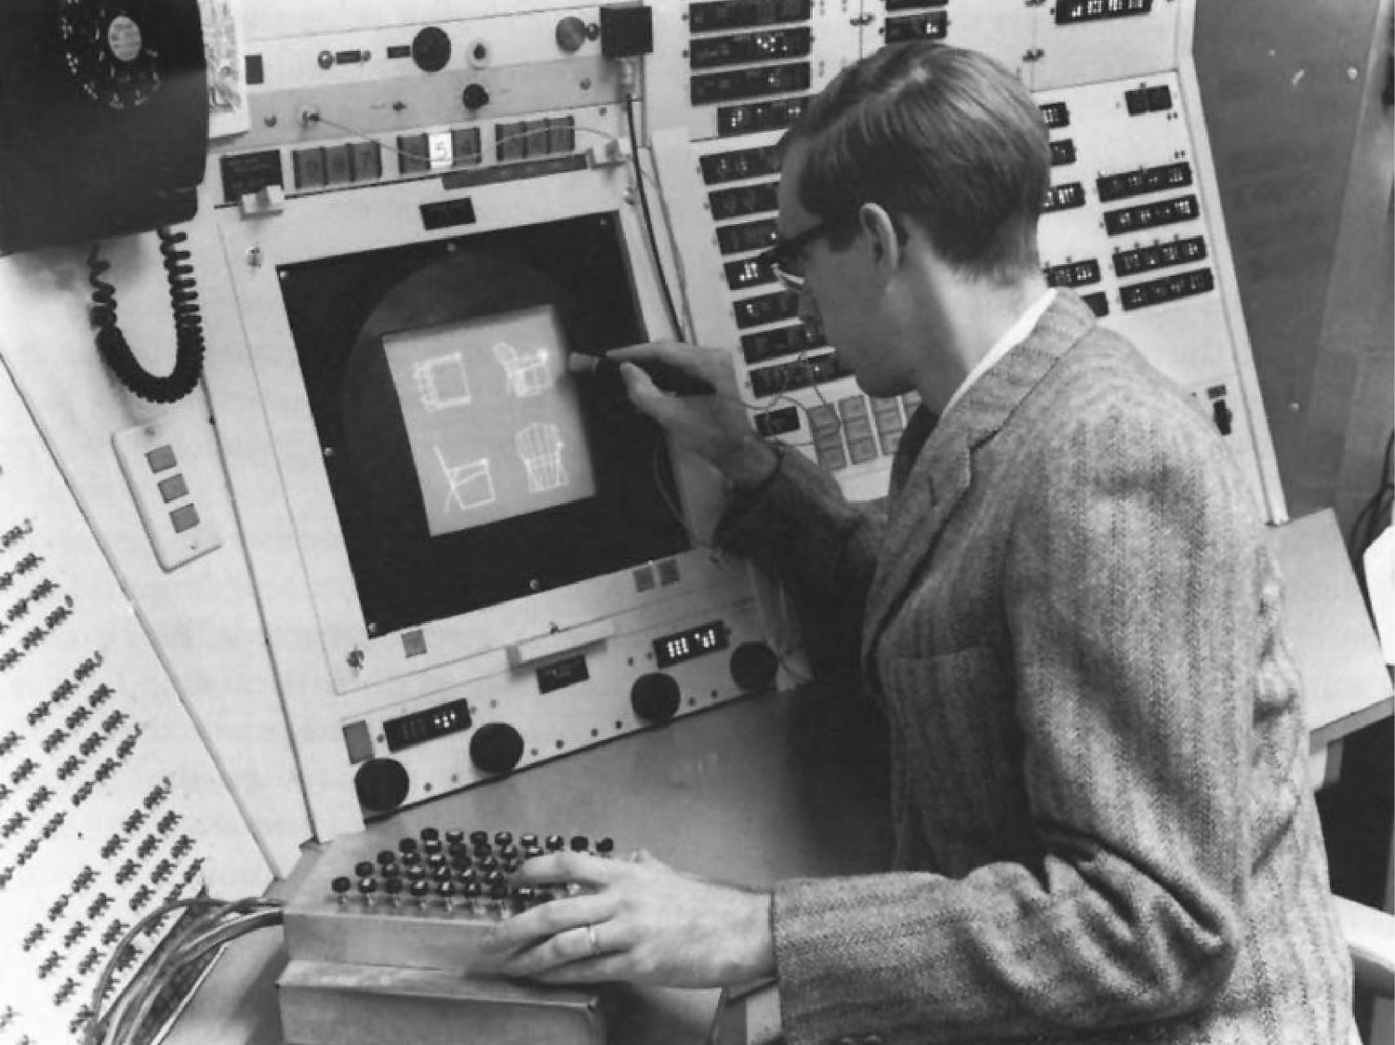
\includegraphics[width=1\textwidth]{chapters/introduction/figures/sketchpad.png}
            \end{center}
            \caption{Sutherland, "Sketchpad" (1963) \cite{sutherland1964sketchpad}}
            \label{fig:sketchpad}
        \end{figure}

        The following systems were designed for collaboration in urban-planning using computational methods and web-based interaction. \textit{Sketchpad} \cite{Sutherland1963}, created at MIT by Ivan E. Sutherland in 1964, is considered the first computer program to use a Graphical User Interface as well as the first multipurpose CAD tool. Major CAD and 3D programs, as well as Object Oriented Programming, HCI systems, interfaces, and data-visualization, sprang from the ideas introduced in Sketchpad and later works by Sutherland. One of Sketchpad's key inventions was the introduction of interactive computing to designers who had no technical knowledge: \textit{``The Sketchpad system makes it possible for a man and a computer to converse rapidly... In the past, we have been writing letters to rather than conferring with our computers.''} \cite{Sutherland1963}
        \newline
        \textit{CommunityViz} \cite{walker2017planners} began in the late 1990's as a software solution to make planning processes more accessible to ordinary citizens. CommunityViz is designed as a decision-support framework, comprising of design and analysis of alternative development scenarios, visualization of design alternatives, analysis of development policies and their impacts over time. A notable implementation of CommunityViz was in the \textit{The Environmental Simulation Center (ESC)} \cite{shakeri2017use}: a NY-based laboratory, which combines computer imaging, policy simulation, and computerized impact analysis to allow citizens to model various site-specific development scenarios. ESC projects involve non-professionals events, where communities and stakeholders join to discuss and learn about the planning process. Lastly, \textit{UrbanSim} \cite{waddell2008urbansim}, an open-source software suite and a service company, has developed tools to engage communities in urban development decision-making, through simulation and visualization. Its main tool, `UrbanCanvas', enables a broad set of users and stakeholders to engage in the planning and design process, build models, and visualize the results.
        \newline
        With the emergence of Augmented Reality technology, some of these systems were translated from 2D to 3D virtual environments. In 2004, \textit{ARTHUR} (Augmented Round Table for Architecture and Urban-planning) \cite{broll2004arthur} was developed in the Bartlett School of Architecture as an interface for urban-design collaboration. Using see-through glasses, ARTHUR generated virtual models of the design setup, allowing members to have equal access to the design scenarios.
        \newline
        The current state of AR technology in commodity devices, and the advancement in marker-less location tracking, has led to a slew of geo-spatial tools and applications, which allow users to interact with virtual objects in real environments \cite{carozza2014markerless}. Popular games like Pokémon-Go and Minecraft helped relink spatial mapping with AR technologies, promoting the development of VR-GIS and AR-GIS systems \cite{boulos2017urban}.
        \newline
        With the emergence of web apps and the increasing move towards Software-As-A-Service model, collaborative WebGIS and online CAD tools proliferated over the internet. Market leaders, such as Autodesk, Google, and Adobe invested in or acquired web applications that allow users to collaboratively work on shared urban models, CAD, and 3D documents, preform spatial analysis, and produce interactive maps, charts, and reports.
        Tools such as Autodesk's Spacemaker \cite{Spacemak73:online}, Google's Delve \cite{DelvebyS33:online}, TestFit \cite{TestFitS86:online}, Hypar \cite{Hypar91:online}, and Archistar \cite{Property12:online} are examples of web-based design platforms that aim to merge traditional CAD, GIS, and spatial-analytics tools into web-based SaaS solutions. A major aspect of these tools is the ability to collaborate using intuitive UI/UX, near real-time analysis, and interoperability between different applications, data structure, and file formats.
    }

    \subsection{Tangible User Interfaces}
    {
        Tangible User Interfaces (TUI) are physical-digital systems in which interaction happens between digital information and physical environments, objects, and devices \cite{Ishii2008}. In the context of UHCI, several TUI pioneered city-planning process which merged physical city-models with computational analysis. In 1970, the MIT Architecture Machine Group (AMG)\footnote{AMG was established to connect architecture, engineering, and artificial intelligence, with projects such as the `URBAN-5', the `Spatial Data Management System', the `Media Room', and the `Aspen Movie Map', a predecessor to Google Street-View application \cite{negroponte1970architecture, negroponte1975soft}.} created a robotic urban TUI installation called \textit{`SEEK'} \cite{negroponte1975soft}. `SEEK' (also referred to as `Blocksworld') featured a computer-controlled environment of small blocks, inhabited by live gerbils. Following a programmed instructions set, the robotic arm rearranged the blocks in predetermined patterns. Once the arrangement was disrupted by the gerbils, the robotic arm would rebuild the block configurations in a manner its programmers believed followed the gerbil's objectives.
        \newline
        A 1972 article described `SEEK': \textit{``Can a computer be programmed to respond intelligently to unexpected events? A toy-block ``city'' was the stage for an experimental contest between a simple computer system named SEEK and a small colony of gerbils. The computer's instructions were to keep the ``city'' in order, but the playful gerbils would not cooperate...''}(Electronics Australia, September 1972). In general terms, SEEK envisioned HCI systems, in which a dialogue between designers and an artificial intelligence system occurs \textit{``not just to solve engineering problems, but to interact with the architect and discuss urban-design problems with him. The computerized environment exhibit was an attempt at showing the problems encountered when living things...interact with a machine which is an integral part of their environment.''} \cite{negroponte1975soft}

        \begin{figure}[h]
            \begin{center}
                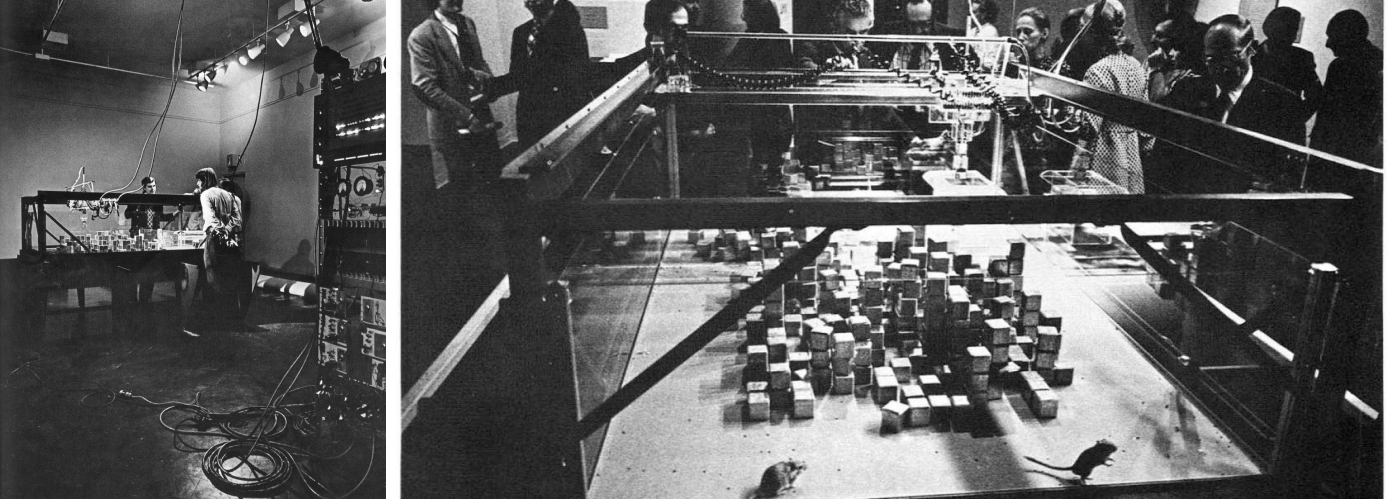
\includegraphics[width=1\textwidth]{chapters/introduction/figures/seek.png}
            \end{center}
            \caption{Negroponte, "URBAN 5: SEEK" (1970) \cite{negroponte1970architecture,negroponte1975soft}}
            \label{fig:seek}
        \end{figure}

        In the following decade, a series of projects sought to enhance and simplify complex design and planning processes: \textit{``TUI represented a new way...of ubiquitous computing by weaving digital technology into the fabric of the physical environment...TUI make digital information directly manipulatable with our hands and perceptible through our peripheral senses through its physical embodiment.''} \cite{Ishii2008} Around the turn of the century, a burst of TUI projects with applications to city-planning emerged from these research groups; The Clay Table, The I/O bulb, the Luminous Room, Augmented Urban-planning Workbench, URP, and LPT and others were created around the same time by researches from MIT School of Architecture and The MIT Media Lab \cite{ishii2002augmented, Ishii2008, Infoscapes, ben-joseph2001, Ullmer2010}.


        \begin{figure}[h]
            \begin{center}
                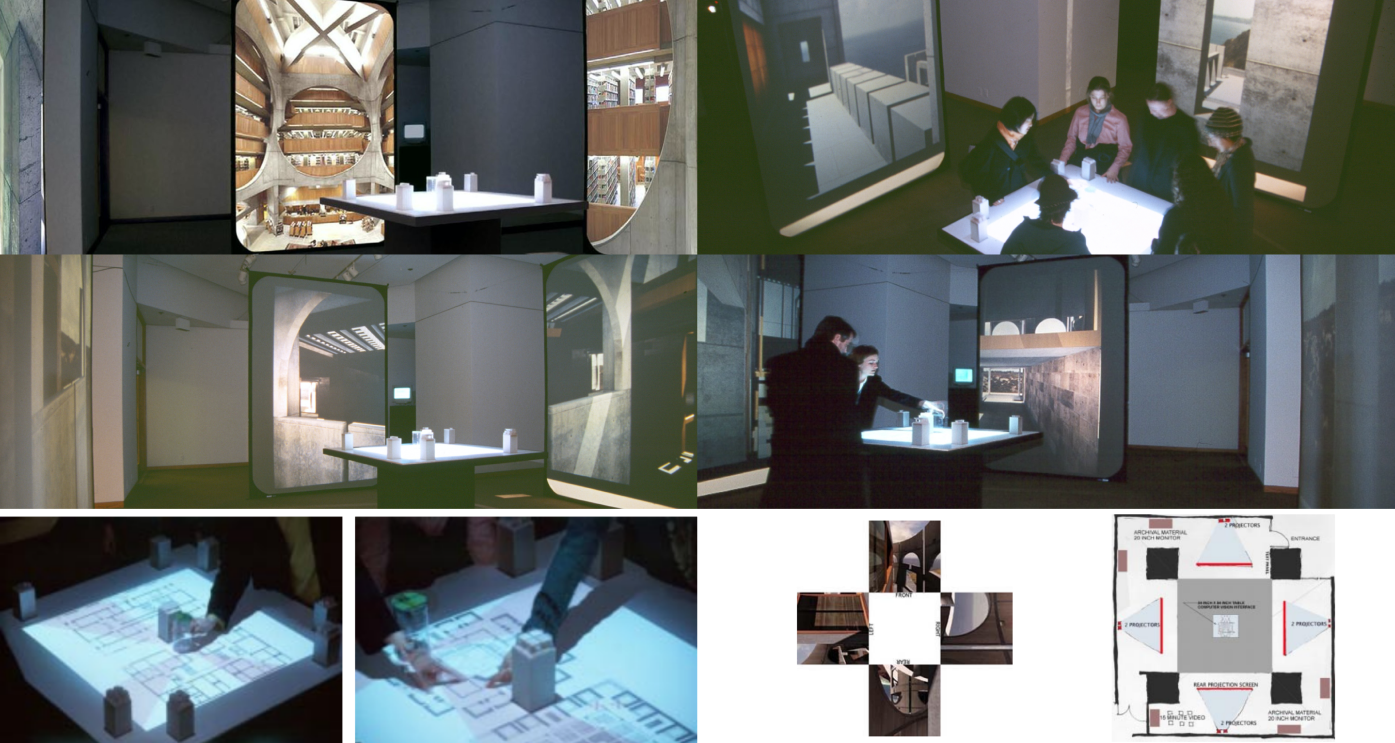
\includegraphics[width=1\textwidth]{chapters/introduction/figures/larson.png}
            \end{center}
            \caption{Larson, "Louis I. Kahn: Unbuilt Masterworks" (1999) \cite{larson2000louis}}
            \label{fig:larson}
        \end{figure}

        The Augmented Urban-planning Workbench \cite{ben-joseph2001} addressed the issue of \textit{``spatial and temporal separation between the varying forms of representation used in urban-design.''} The system included a table with a physical city-model, and a projection scheme of different analysis layers, such as sun-shade, traffic simulation, and architectural geometry. The Workbench saw the inconsistency of design representation as critical bottleneck for successful collaboration amongst stakeholders: \textit{``By `triangulating' between these multiple forms of representation, we gain a more realistic sense of the site and proposed urban-design.''} \cite{ben-joseph2001}
    }

    \section{Discussion: UHCI}
     {
      Over the past few decades, different UHCI solutions were suggested in order to transcend lengthy, inefficient, and costly city-planning processes. Advancements in AI and Data Science could supercharge these systems with real-time, high-end urban analytics \cite{Batty2013, Kitchin2014}. Affordable computation and immersive technology, such as AR or VR, can help better communicate design alternatives, their impacts and tradeoffs \cite{shakeri2017use,banerjee2011companion}.
      \newline
      Despite its promise, with the emergence of every new technology new challenges arise, and some issues still remain. This section discusses some of these challenges, specifically (i) technical limitations, accuracy or bias in models and data, (ii) the potential perils of `techno-utopia' and over-reliance on technology, and (iii) the accessibility and technical literacy of designers, stakeholders, and the community.


      \subsection{Technical and Access Limitations}
      {
          The majority of previously presented UHCI platforms are designed around the exploration of the city's physical aspects \cite{ben-joseph2001}. More implicit themes, such as inequality, urban economics, social, health or cultural aspects, might not be easily integrated into these technologies \cite{Snyder2003}. As a result, discussions might be focusing on the physical aspects, while neglecting less tangible issues: \textit{``The spatial and temporal separation between the forms of design representation increases the cognitive load...The urban-designer is in critical need of a platform that allows the simultaneous understanding of a wide variety of representations...''} \cite{ben-joseph2001}
          Moreover, the design of UHCI platforms emphasizes simplification, readability, and the user experience \cite{Ishii2008}. This can result with a degree of over-simplification that omits information in favor of usability. Specifically, platforms that favor tangible interactions might limit the breadth of design exploration, so that only a curated set of predefined use-cases could be explored \cite{mahyar2016ud}. The tradeoffs between usability, simplicity and oversimplification must be addressed in the inception of technology-driven urban processes.
          \newline
          A similar risk is data overload and information saturation. The sheer volume of data, analysis, and visualizations presented in these systems might be inspiring for technical consumers, but might overwhelm others \cite{Snyder2003}. Technophobia and resentment could arise from systems that appear overly complex, or if the goals are not clear \cite{innes2010planning}. This also relates to the cultural divide between prospective participants and users of these tools. Even though the ubiquity of computation puts powerful devices in the hands of billions, there are still significant portions of society that cannot effectively make use of new technologies \cite{Innes2016, brusaporci2017importance}. Certain design decisions, terminological terms, and even color schemes, can cause unintentional bias and hinder interaction. The design of new participatory processes must aim to engage the majority of the public, and constantly improve the tools' legibility, coherence and accessibility through feedback.
      }

      \subsection{Challenges of UHCI-Based Processes}\label{intro:challanges-processes}

      {
          UHCI platforms do not necessarily bear the promise of a `better urban process'. In some cases, new technologies might be adapted by decision makers for the sole purpose of creating a false impression of engagement and collaboration \cite{Innes2016, banerjee2011companion}. Even in democratic processes, over-bureaucratization, privatization and self-interests can still discourage citizens from involvement.
          Additionally, growing concerns around surveillance, privacy, and algorithmic injustice, may also challenge technology-driven processes \cite{green2019smart}. Although some data and models could emerge from publicly available resources, high-quality and high-resolution data are still mostly proprietary and limited, which might hinder privacy advocates from active participation \cite{Barbosa-Filho2017}.
          \newline
          Moreover, reliance on UHCI platforms for decision-making processes could shift the balance between decision-makers, design professionals and the general public \cite{ben-joseph2001, mueller2018citizen}. Although meant to increase transparency and just distribution of public resources, it is possible that powerful public advocacy could find loop-holes and edge-cases in such systems. As Hester argues, this kind of ``adversarial planning'' could create uninspiring places and perpetuate urban status-quos \cite{hester2006design}. It is therefore crucial that the tools are conceived so that a mutual search for ``better design'' would be their main motivation \cite{banerjee2011companion}.
          \newline
          Amidst these challenges, it is necessary for UHCI technologies to be included in an holistic planning process, and not just as merely `educational' tech-props in public sessions. As Arenstein concludes, information and data sharing are important steps towards meaningful participation, but cannot substitute the distribution of real decision-making power \cite{arnstein1969ladder}. What Innes describes as ``Collaborative Participation'' could be achieved when the design of the process itself is open to critical review, and the participating parties propose their own data, models and results \cite{Innes2016}. Engaging the public in the inception, co-creation, and development of these tools will also increase their transparency, and reduce the ``cultural shock'' associated with new technologies \cite{banerjee2011companion}. If successful, members of the public who would take active roles in co-creation efforts, would become ambassadors of this new urban process.
      }
     }

    %%%%%%%%%%%%%%%%%%%%%%%%%%%%%%%%%%%%%%%%%%%%%%%%%%%%%%%%%%%%%%%%%%%%%%%%%%%%

    \section{CityScope: A New Urban Process}
     {
      As discussed in previous sections, the need for a new urban process is becoming globally recognized, and is being addressed by new policies, strategies, and technologies: \textit{``(we) presents a paradigm shift based on the science of cities; it lays out standards and principles for the planning, construction, development, management, and improvement of urban areas...foster the creation...of open, user-friendly and participatory data platforms using technological and social tools available to transfer and share knowledge...to enhance effective urban-planning and management.''} \cite{habitat2016new}.
      \newline
      This dissertation proposes a new urban-planning and decision-making process through the design, development, and deployment of \textbf{CityScope}: an urban modeling, simulation and decision-making platform. CityScope is an on-going research project at the MIT Media Lab City Science Group, that offers a wide range of technologies to meet planning questions from a human-centric point of view. The rest of this section describes the structure of this dissertation, and the main themes leading the development of CityScope.
     }

    \begin{figure}[!htb]
        \begin{center}
            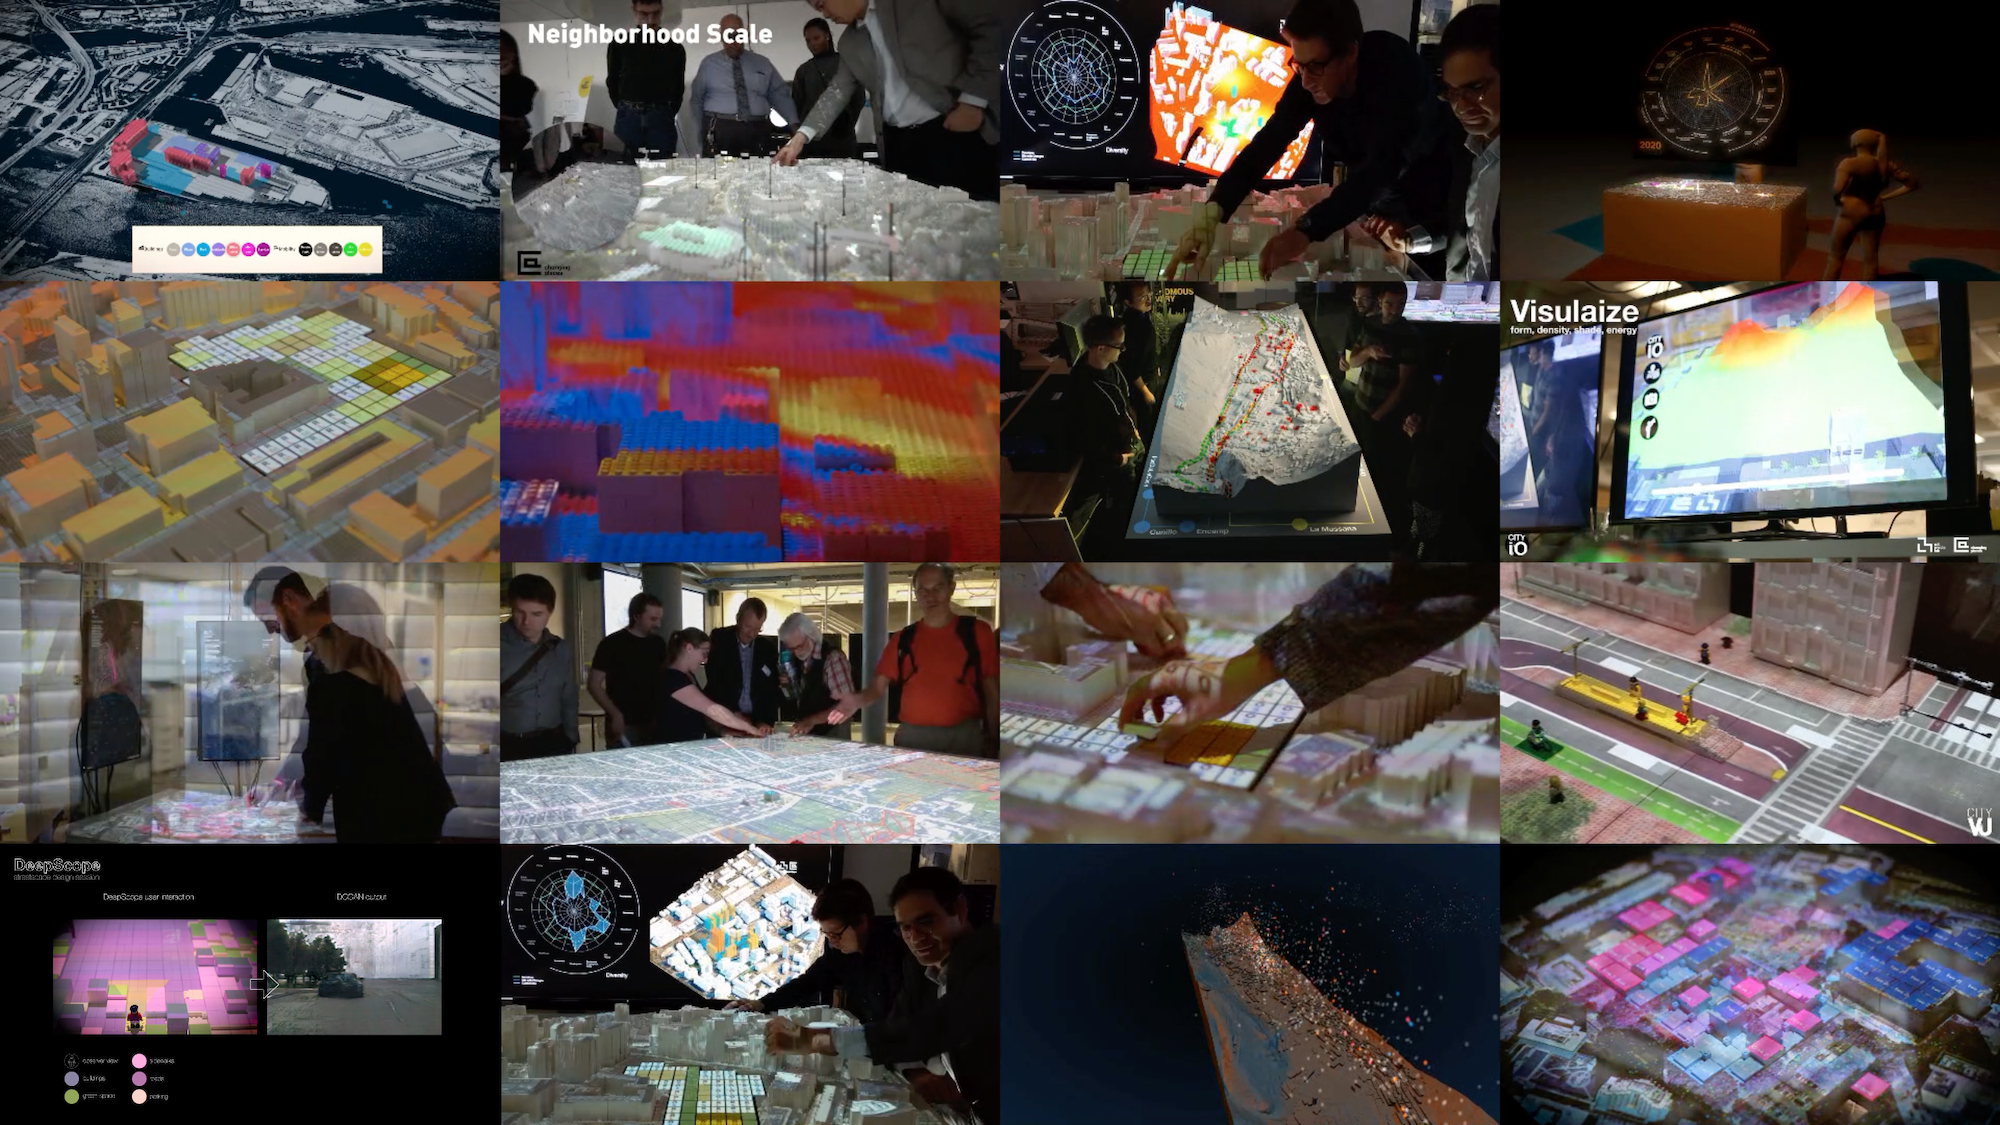
\includegraphics[width=1\linewidth]{chapters/introduction/figures/all_projects.png}
        \end{center}
        \caption{CityScope projects and deployments(from top left): Grasbrook, Boston BRT Neighborhood, Volpe, Champs-Elysees, Volpe, Urban Observatory, Andorra, csAR, MoCho, FindingPlaces, Volpe, Boston BRT Street, DeepScope, Volpe, Reversed Urbanism, MoCho}
        \label{fig:all_projects}
    \end{figure}

    \subsection{CityScope Themes}
    {
        CityScope is being developed over the past decade at MIT as well as by research labs, companies, and individuals around the world. This thesis clusters the many prototypes, systems, platforms, deployments, and milestones of CityScope into four major themes: \textbf{Insight}, \textbf{Transformation}, \textbf{Prediction} and \textbf{Consensus}. These themes are described below; The rest of this chapter lists CityScope's milestones, key publications, and contributions.


        \subsubsection{Chapter \eqref{ch:insight}: Insight}
        {
            Insights are key in the understanding of current and past state of urban systems. New spatial analytics and urban-modeling techniques, novel data resources, as well as new processing methodologies can support planning processes with high-quality insights \cite{salganik_bit_2017, Kitchin2014, ben-joseph2001}. The first chapter of this thesis discusses CityScope role as an urban observatory, using methods of urban and spatial analytics, and focusing on high-resolution, geo-located, urban dynamics.
        }

        \subsubsection{Chapter \eqref{ch:transformation}: Transformation}
        {
            Interactive technologies, including Virtual, Augmented, and Mixed Reality, Computer-Vision, Tangible Interfaces, as well as web applications, can support iterative and participatory urban processes. These technologies provide playful and exploratory environment to examine counterfactual scenarios. Design iterations could simultaneously be evaluated for their tradeoffs and Key Performance Indicators (KPIs) \cite{Ben-Joseph2013, Ben-Joseph2004,Ishii2008}. Data-driven methods can expedite the investigation of complex planning scenarios and their effects on human dynamics, traffic, energy-use, or economic performance \cite{Foth2011, Song2010}.
            The second chapter of this thesis describes the role of CityScope as a tool for urban transformation, focusing on the design, development, and usage of various UHCI systems.
        }

        \subsubsection{Chapter \eqref{ch:prediction}: Prediction}
        {
            Interventions in the built environment are lengthy, closely, and have tremendous impact on the lives of communities and individuals. Urban predictions are therefore necessary for risk mitigation and impact assessment \cite{batty2013new, Glaeser2011, Song2010}. In recent years, new methods of urban simulation, data-driven models, Machine Learning, and real-time data allow for the investigation of more implicit urban phenomenons. The third chapter of this thesis describes the role of CityScope for urban prediction, focusing on the development of UHCI simulation and forecasting systems of implicit aspects of the built environment.
        }

        \subsubsection{Chapter \eqref{ch:consensus}: Consensus}
        {
            Engaging multiple stakeholders in urban decision-making is a fundamental aspect in a new urban process \cite{habitat2016new, banerjee2011companion}. Unlike traditional processes, new consensus-building tools can be designed around large-scale, physical or virtual spaces, that facilitate city-wide participation and decision-making. They can reduce the bureaucratic overhead of negotiating in different channels, and promote concise and result-driven discussions \cite{ben-joseph2001, habitat2016new, Innes2016}.
            The last chapter of this thesis describes the role of CityScope as a tool for urban consensus, focusing on the development of UHCI systems for multi-stakeholder decision-making, policy recommendations, and the facilitation of collaborative decision-making.
        }


        \begin{figure}[!htb]
            \begin{center}
                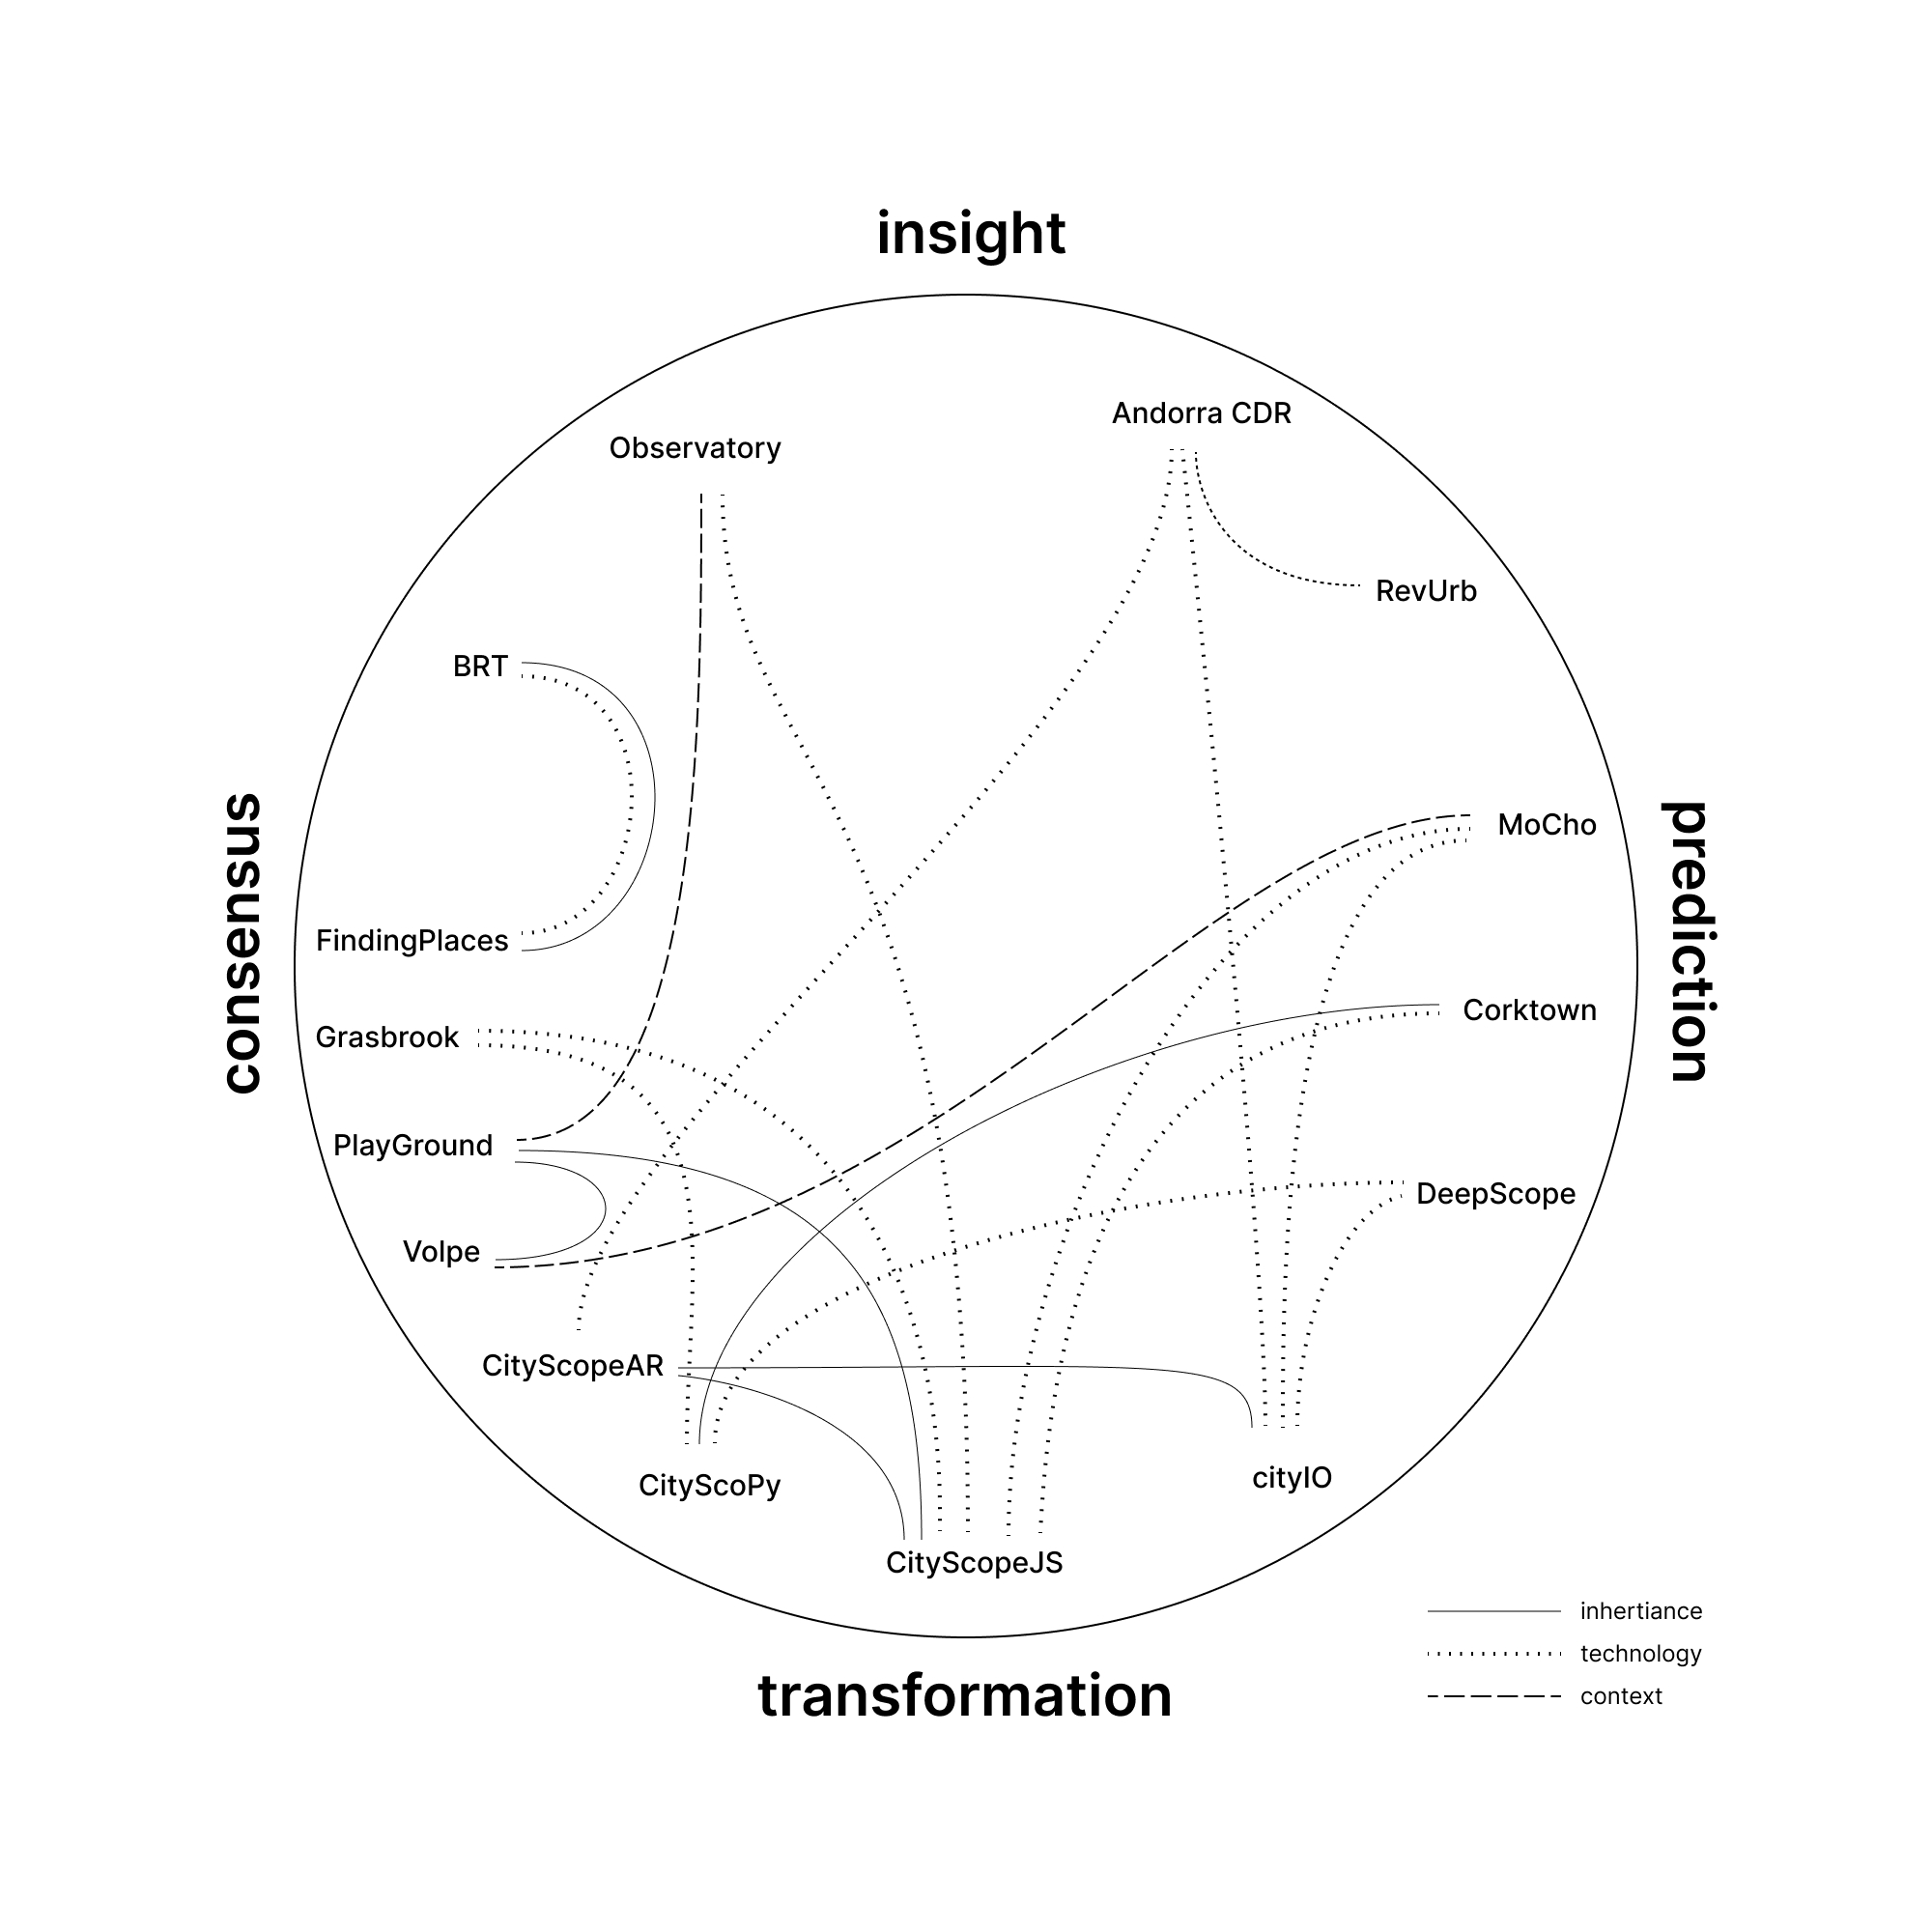
\includegraphics[width=1\textwidth]{chapters/introduction/figures/projects_relations.jpg}
            \end{center}
            \caption{
                Relations between projects, publications, and deployments of the CityScope platform. In this diagram, projects appearing in this thesis are approximated to their corresponding theme, and are linked to other projects through three types of relations: \textit{Inheritance:} project was built upon the thematic ideas and learning outcomes of previous work; \textit{Technology:} project made use of technological advancement achieved in prior work; and \textit{Context:} project was built in a similar context (geographical location, time period, research question, etc.).
            }
            \label{fig:projects_relations}
        \end{figure}
    }
    %%%%%%%%%%%%%%%%%%%%%%%%%%%%%%%%%%%%%%%%%%%%%%%%%%%%%%%%%%%%%%%%%%%%%%%%%%%%%%%%%%%%%%%%%%%%%%%%%%%

    \section{Contributions}
 {
  This thesis contributes to urban modeling and simulation, HCI, Decision Support Systems, urban decision-making and consensus-building in several aspects:

  \begin{itemize}
        \item The development of a scalable, real-time, socio-technical urban modeling and simulation platform.
        \item The development of a system and a schema for urban analytics through distributed computation system.
        \item The development of real-time, explicit and implicit spatial analytics modules to asses urban behavior, mobility, and performance.
        \item Deployment of dozens of CityScope platforms around the world, some of which in real-world city-planning contexts.
        \item The creation of community of users, developers, contributes, and researchers building and using CityScope worldwide.
  \end{itemize}
 }

\section{Publications, Projects, and Deployments}\label{sec:publications-projects-deployments}

{
      The following is a list of publications, projects, and deployments of the CityScope platform, as well as corresponding research in Urban Sciences, Spatial Analytics, and mutual fields.

      %%%%%%%%%%%%%%%%%%%%%%%%%%%%%%%%%%%%%%%%%%%%%%%%%%%%%%%%%%%%%%%%%%%%%%%%%%%%%%%%%%%%%%%%%%%%%

      {
\textbf{Noyman, A.}, Larson, K. (2020, April). DeepScope: HCI Platform for Generative Cityscape Visualization. In Extended Abstracts of the 2020 CHI Conference on Human Factors in Computing Systems (pp. 1-9).
}

{
\textbf{Noyman, A.}, Doorley, R., Xiong, Z., Alonso, L., Grignard, A., Larson, K. (2019). Reversed urbanism: Inferring urban performance through behavioral patterns in temporal telecom data. Environment and Planning B: Urban Analytics and City Science, 46(8), 1480-1498.
}

{
Doorley, R., \textbf{Noyman, A.}, Sakai, Y., Larson, K. (2019). What's your MoCho? Real-time Mode Choice Prediction Using Discrete Choice Models and a HCI Platform.
}

{
Alonso, L., Zhang, Y. R., Grignard, \textbf{A., Noyman}, A., Sakai, Doorley, R., Y., ElKatsha, M., Larson, K. (2018, July). Cityscope: a data-driven interactive simulation tool for urban-design. Use-case volpe. In International conference on complex systems (pp. 253-261). Springer.
}

{
\textbf{Noyman, Ariel}, Yasushi Sakai, and Kent Larson. "Cityscope{AR}: urban-design and crowdsourced engagement platform." arXiv preprint arXiv:1907.08586 (2019).
}

{
Grignard, A., Macià, N., Alonso Pastor, L.,\textbf{Noyman, A.}, Zhang, Y., Larson, K. (2018, July). Cityscope andorra: A multi-level interactive and tangible agent-based visualization. In Proceedings of the 17th International Conference on Autonomous Agents and MultiAgent Systems (pp. 1939-1940).
}

{
\textbf{Noyman, A.}, Holtz, T., Kröger, J., Noennig, J. R., Larson, K. (2017). Finding places: HCI platform for public participation in refugees’ accommodation process. Procedia computer science, 112, 2463-2472.
}

{
Alrashed, T., Almalki, A., Aldawood, T., \textbf{Noyman, A.}, ... Alwabil, A. (2015). An observational study of usability in collaborative tangible interfaces for complex planning systems. Procedia Manufacturing, 3, 1974-1980.
}

{
\textbf{Noyman, A.} (2015). POWER/STRUCTURES: the Urban Form of Regulations (SM Thesis, Massachusetts Institute of Technology).
}

      %%%%%%%%%%%%%%%%%%%%%%%%%%%%%%%%%%%%%%%%%%%%%%%%%%%%%%%%%%%%%%%%%%%%%%%%%%%%%%%%%%%%%%%%%%%%%

      \begin{rotatepage}
    \begin{landscape}

        \subsection{CityScope Projects and Deployments}
        {
            The following list (see Table \eqref{table:intro_cs_projects}) includes major CityScope projects developed at MIT, and deployed in real-world use-cases. Since its inception in 2013, and especially since CityScope was open-sourced in 2016, many instances of the TUI, backend, frontend, software, or hardware were developed, deployed, or used around the world. This list is therefore a non-exhaustive attempt to highlight key contributions and the many contributes who supported CityScope development. When academic publications were available, contributes were cited in the order they appear; In other cases, the MIT Media Lab website served as a source of information; Lastly, blog posts and other unverified sources of information were used to supplement the list.
        }


        \scriptsize
        \begin{longtable}
            {>{\raggedright}p{0.2\textwidth}>{\raggedright}p{0.2\textwidth}p{0.1\textwidth}p{0.2\textwidth}p{0.1\textwidth}p{0.6\textwidth}}
            \caption[CityScope Projects]
            {
                \bigskip
                CityScope Projects, Deployments, and Academic Activities.
                \newline
                \scriptsize Legend:\textbf{(*)}: Project is detailed in this thesis; \textbf{WEB}: Web-based tool, most commonly CityScopeJS; \textbf{SW}: Software tool or backend module; \textbf{MR}: Mixed-reality, using augmented or virtual reality hardware; \textbf{TUI}: tangible User Interface; \textbf{CSL}: deployment in one or many City Science Labs; \textbf{CSN}: Members of the City Science Network; \textbf{ML}: MIT Media Lab, City Science group.
                \bigskip
            }
            \label{table:intro_cs_projects}                                                                                                                                                                                                                                                                                                                                                                                                                   \\

            \textbf{PROJECT}                                                 & \textbf{DESCRIPTION}                                    & \textbf{MEDIUM} & \textbf{DEPLOYMENT}      & \textbf{YEAR} & \textbf{TEAM}                                                                                                                                                                                                                                           \\
            \hline
            \endfirsthead

            \textbf{PROJECT}                                                 & \textbf{DESCRIPTION}                                    & \textbf{MEDIUM} & \textbf{DEPLOYMENT}      & \textbf{YEAR} & \textbf{TEAM}                                                                                                                                                                                                                                           \\
            \hline
            \endhead

            Urban Prototyping                                                & City Science IAP course                                 & TUI             & ML                       & `13           & Ryan CC Chin, Michael Lin, Ira Winder, Kent Larson                                                                                                                                                                                                      \\
            Projection Mapping\cite{Inventin89:online}                       & Projection Mapping prototype using Lego                 & TUI             & ML                       & `13           & Michael Lin, Kent Larson                                                                                                                                                                                                                                \\
            CityScope Riyadh\cite{aldawood2014interaction}                   & Daylight, energy, and walkability modeling              & TUI             & Riyadh                   & `13-`15       & Almaha Almalki, Anas Alfaris, Areej Al-Wabil, Christoph Reinhart, Cody Rose, Faisal S. Aleissa, Ira Winder, Julia Sokol, Kent Larson, Mohammad Hadhrawi, Salma Aldawood, Tarfah Alrashed (KACST)                                                        \\
            CityScope Kendall(*)\cite{Hadhrawi2016}                          & Urban-data observatory                                  & TUI             & ML                       & `13-`16       & Mohammad Hadhrawi, Ira Winder, Carson Smuts, JT White, Luis Alonso, Ryan CC Chin, Suramya Kedia, Sitorios Kotsopoulos, Estelle Yoon, Ariel Noyman, Kent Larson                                                                                          \\
            CityScope LUT                                                    & Land use and transportation planning                    & TUI             & Toronto                  & `15           & Ira Winder, Carson Smuts, Kent Larson                                                                                                                                                                                                                   \\
            CityScope Playground(*)\cite{noyman2015powerstructures}          & Dynamic zoning simulator                                & TUI             & APA, Cambridge           & `14-`15       & Ariel Noyman, Lezhi Li, Wei Lin, Ira Winder, Kent Larson                                                                                                                                                                                                \\
            CityScope BRT(*)\cite{Newinter52:online}                         & BRT solutions for Boston metro area                     & TUI, SW         & Boston                   & `14-`15       & Anson F. Stewart, Ariel Noyman, Phil Tinn, Jeffrey L. Rosenblum, Christopher Zegras, Kent Larson, Ryan CC Chin, Nuestra Comunidad, DUSP - Mobility Futures Collaborative                                                                                \\
            CityScopeAR(*)\cite{noyman2018CityScopeARUD}                     & Mixed-Reality platform for urban modeling               & MR, SW          & Andorra, Volpe, BRT, APA & `15-`18       & Ariel Noyman, Yasushi Sakai, Nikita Samsonov, Kent Larson                                                                                                                                                                                               \\
            CityScope FindingPlaces(*)\cite{Noyman2017FP}                    & Refugees' accommodation participation process           & TUI             & Hamburg                  & `15-`16       & Ariel Noyman, Tobias Holtz, Johannes Kroger, Nina Halker, Katrin Hovy, Gesa Ziemer, Kent Larson                                                                                                                                                         \\
            cityIO(*)\cite{noyman2018CityScopeARUD}                          & CityScope backend server                                & SW              & ML, CSL                  & `16-present   & Yasushi Sakai, Nikita Samsonov (CSAIL), Ariel Noyman                                                                                                                                                                                                    \\
            CityScope Andorra(*)\cite{Grignard:2018:CAM:3237383.3238030}     & Urban simulation for Andorra                            & TUI             & Andorra                  & `16-`17       & Luis Alonso, Arnaud Grignard, Ariel Noyman, Ryan Zhang, Dalma Foldesi, Jung In Seo, Juanita Devis, Núria Macià (Fundació ActuaTech), Marc Vilella (OBSA), Marc Pons (OBSA), Guillem Francisco Giné (OBSA), Cristina Yañez (UdA), Kent Larson            \\
            CityScope Andorra CDR(*)\cite{Grignard:2018:CAM:3237383.3238030} & Urban mobility data observatory for Andorra             & TUI             & Barcelona Smart Cities   & `16           & Luis Alonso, Arnaud Grignard, Ariel Noyman, Ryan Zhang, Núria Macià (Fundació ActuaTech), Marc Vilella (OBSA), Marc Pons (OBSA), Guillem Francisco Giné (OBSA), Cristina Yañez (UdA), ACTUA Tech, Kent Larson                                           \\
            CityScope Volpe(*)\cite{alonso2018cityscope}                     & Urban simulation for the Volpe development site         & TUI             & ML                       & `16-present   & Luis Alonso, Ryan Zhang, Arnaud Grignard, Ariel Noyman, Yasushi Sakai, Markus ElKatsha,  Ronan Doorley, Kent Larson                                                                                                                                     \\
            CityScope LivingLine                                             & Sensing commercial street performance                   & TUI             & Shanghai, ML             & `17-`20       & Ryan Zhang, Yang Liu, Thomas Sanchez Lengeling, Luis Alonso, Chenhan Jiang, Markus Elkatsha, Weiting Xiong, Tianyu Su, Tianyi Fan, Will Shun Du, Xingda Guo, Kent Larson                                                                                \\
            Hamburg PortCity Model\cite{lopez2019testing}                    & Mobility ABM tool for Cruise Passenger transfer         & SW              & Hamburg                  & `17-`20       & Jesús López Baeza, Jörg Rainer Noennig, Vanessa Weber, Arnaud Grignard, Ariel Noyman, Kent Larson, Sebastian Saxe, Ulrich Baldauf                                                                                                                       \\
            CityScope Aalto                                                  & Planning platform for the Aalto Campus in Otaniemi      & SW, WEB, TUI    & Aalto University         & `17-`19       & Ronan Doorley, Ariel Noyman, Arnaud Grignard, Kent Larson, Eetu Ristaniemi (Aalto), Jarmo Suominen (Aalto), Antti Ahlava (Aalto), Antti Tuomela (Aalto), Anssi Joutsiniemi (Aalto)                                                                      \\
            Reversed Urbanism(*)\cite{noyman_inpress}                        & Human behavioral patterns using telecom data            & WEB             & ML                       & `18           & Ariel Noyman, Ronan Doorley, Zhekun Xiong, Luis Alonso, Arnaud Grignard, Esteban Moro, Kent Larson                                                                                                                                                      \\
            CityScope MoCho(*)\cite{doorley2019s}                            & Mobility Mode Choice modeling platform                  & WEB             & ML                       & `19           & Ronan Doorley, Ariel Noyman, Yasushi Sakai, Kent Larson                                                                                                                                                                                                 \\
            CityScope DeepScope(*)\cite{noyman2020deepscope}                 & Generative urban visulization platform                  & TUI             & ML                       & `19           & Ariel Noyman, Kent Larson                                                                                                                                                                                                                               \\
            CityScopeJS(*)                                                   & CityScope Distributed web platform                      & WEB             & ML, CSL                  & `18-present   & Ariel Noyman, Yuke Zheng (CSAIL), Ronan Doorley, Luis Alonso, Arnaud Grignard, Yasushi Sakai, Markus ElKatsha, Kent Larson                                                                                                                              \\
            CityScope Champs-Élysées(*)                                      & Simulating interventions impact for the Champs-Élysées  & TUI             & Paris                    & `19-`20       & Arnaud Grignard, Nicolas Ayoub, Luis Alonso, Ariel Noyman, Markus Elkatsha, Maggie Church, Kent Larson, Tri Nguyen-Huu (IRD), Patrick Taillandier (INRA), Alexis Drogoul (IRD)                                                                          \\
            RoboScope                                                        & CityScope robotic interface                             & TUI             & ML                       & `18-present   & Markus ElKatsha, Thomas Sanchez Lengeling, Kent Larson                                                                                                                                                                                                  \\
            CityScope Corktown(*)                                            & Simulating planning and mobility scenarios              & SW, WEB         & Detroit                  & `19-`20       & Ronan Doorley, Ariel Noyman, Luis Alonso, Can Wang, Arnaud Grignard, Cristian Jara-Figueroa, Yasushi Sakai, Kent Larson, Ford Company                                                                                                                   \\
            CityScope Grasbrook(*)\cite{baeza2021cityscope}                  & Platform for evaluating design competition proposals    & TUI             & ML, Hamburg              & `18-present   & Jesus Lopez Baeza, Julia Sievert, Andre Landwehr, Jonas Luft, Philipp Preuner, Jurgen Bruns-Berentelg, Ariel Noyman, Joerg Rainer Noennig, Kent Larson, Gesa Ziemer                                                                                     \\
            CS-BRIX(*)                                                       & CityScope modules communication library                 & SW              & ML, CSL                  & `19-`21       & Cristian Ignacio Jara Figueroa, Ariel Noyman, Kent Larson                                                                                                                                                                                               \\
            CityScope Cooper Hewitt                                          & Exhibit at the Cooper Hewitt, The Road Ahead exhabition & TUI             & ML, New York City        & `18           & Gabriela Bila Advincula, Carson Smuts, Yasushi Sakai, Ryan Zhang, Ariel Noyman, Ronan Doorley, Arnaud Grignard, Alex Berke, Guadalupe Babio Fernandez, Markus Elkatsha, Luis Alberto Alonso Pastor, Maitane Iruretagoyena, Margaret Church, Kent Larson \\
            CityScope Vietnam                                                & Ho Chi Minh City `District 4'                           & WEB, TUI        & ML, CSL                  & `20-present   & Ariel Noyman, Ryan Zhang, Ronan Doorley, Luis Alonso, Thomas Sanchez Lengeling, Arnaud Grignard, Yasushi Sakai, Markus ElKatsha, Kent Larson                                                                                                            \\
            CityScope EPA                                                    & CityScope platfrom for East Palo Alto                   & WEB             & ML, CSL                  & `20-present   & Ronan Doorley, Luis Alonso, Markus ElKatsha, Ariel Noyman, Kent Larson                                                                                                                                                                                  \\
            Jerusalem Workshop                                               & CityScopeJS web platform                                & WEB             & CSN                      & `20           & Ariel Noyman, Ronan Doorley, Yasushi Sakai, Luis Alonso, Ryan Zhang, Cristian Jara Figueroa, Arnaud Grignard, Markus Elkatsha, Thomas Sanchez                                                                                                           \\
            CS Network Workshop                                              & CityScopeJS web platform                                & WEB             & CSN                      & `21           & Ariel Noyman, Ronan Doorley, Yasushi Sakai, Luis Alonso, Ryan Zhang, Cristian Jara Figueroa, Arnaud Grignard, Markus Elkatsha, Thomas Sanchez                                                                                                           \\
        \end{longtable}
    \end{landscape}
\end{rotatepage}

}



\subsection{CityScope Milestones}

{This list includes CityScope milestones, exhibitions, awards, and mentions in the press and popular media:

      \begin{itemize}

            \item{CityScope was featured in “Report to The President - Technology and the Future of Cities”, President's Council of Advisors on Science and Technology, 2016 (pp. 23)}

            \item{CityScope project presented in the `Road Ahead' exhibition at the Cooper Hewitt Museum, NYC, 2019.}

            \item{“FindingPlaces”: Public participation process using CityScope for data-driven housing allocation and planning for 80,000 refugees}

            \begin{itemize}
                  \item{
                              OECD Observatory for Public Sector Innovation (OPSI) and the United Arab Emirates (UAE) Mohammed Bin Rashid Centre for Government Innovation (MBRCGI) selected “FindingPlaces” out of 600 submission as a `Global Innovation': \url{https://trends2019.oecd-opsi.org/}
                        }

                  \item{
                              “FindingPlaces” won the United Nations - “Urban Act Award”, \url{https://urbact.eu/finding-places}
                        }
            \end{itemize}

            \item{
                        Poon, L. (2015, October 16). MIT's New Interactive LEGO Urban Tool Brings Transparency to Transit Planning. Retrieved July 26, 2020, from \url{https://www.bloomberg.com/news/articles/2015-10-16/mit-s-new-interactive-lego-urban-tool-brings-transparency-to-transit-planning}
                  }

            \item{
                        Gillies, C. (2014, December 18). LEGO: Can this most analogue of toys really be a modern urban-planning tool? Retrieved July 26, 2020, from \url{https://www.theguardian.com/cities/2014/dec/18/lego-toys-urban-planning-tool-architects-mit}
                  }

            \item{
                        Making ideas into reality at MIT's "Future Factory". (n.d.). Retrieved July 26, 2020, from \url{https://www.cbsnews.com/news/60-minutes-mit-media-lab-making-ideas-into-reality-future-factory-2019-08-04/}
                  }

            \item{
                        Rob Matheson | MIT News Office. (2017, October 13). Small European nation becomes a "living lab" for urban innovation researchers. Retrieved July 26, 2020, from \url{http://news.mit.edu/2017/european-nation-andorra-living-lab-media-lab-urban-innovation-1013}
                  }

            \item{
                        Science of Teams: Science of Teams. (2017, January 23). Science of Teams: How MIT Media Lab Builds Cities Using LEGO and Augmented Reality. Retrieved July 26, 2020, from \url{https://www.wired.com/video/watch/science-of-teams-mit-media-lab}
                  }

            \item{
                        Prevost, L. (2018, April 03). Building a Connected City From the Ground Up. Retrieved July 26, 2020, from \url{https://www.nytimes.com/2018/04/03/business/smart-city.html}
                  }

            \item{
                        Wener-Fligner, Z. (2014, December 19). LEGO makes a monochrome set targeted at architects. Retrieved July 26, 2020, from \url{https://qz.com/315776/lego-for-grown-ups-the-toy-maker-is-targeting-architects-and-urban-planners/}
                  }

            \item{
                        GOLDSMITH, BOUSQUET, AR is Transforming Tech. What Can It Do for Cities?. Retrieved July 26, 2020, from \url{https://datasmart.ash.harvard.edu/news/article/ar-transforming-tech-what-can-it-do-cities}
                  }

            \item{
                        LAURA ADLER,. (2016, AUGUST 29). SimCities: Can City-planning Mistakes Be Avoided Through Data-Driven Simulations? Retrieved July 26, 2020, from \url{https://www.govtech.com/data/SimCities-Can-City-Planning-Mistakes-Be-Avoided-Through-Data-Driven-Simulations.html}
                  }

            \item{
                        Garcia, J. (2018, July 08). El MIT usa fichas LEGO y big data para saber dónde dar futuro a los inmigrantes. Retrieved July 26, 2020, from \url{https://www.lainformacion.com/tecnologia/el-mit-salva-inmigrantes-con-fichas-lego-gracias-al-big-data-sabe-donde-deben-ser-situados-en-una-ciudad/6351916/}
                  }

            \item{
                        Woldin, P. (2016, March 02). „City-Scope": Mit Legosteinen Flüchtlingsunterkünfte finden - WELT. Retrieved July 26, 2020, from \url{https://www.welt.de/regionales/hamburg/article152836431/Mit-Legosteinen-Fluechtlingsunterkuenfte-finden.html}
                  }

      \end{itemize}
}

}
%%%%%%%%%%%%%%%%%%%%%%%%%%%%%%%%%%%%%%%%%%%%%%%%%%%%%%%%%%%%%%%%%%%%%%%%%%%%%%%%%%%%%%%%%%%%%%%%%%%





